\documentclass[../main.tex]{subfiles}
\graphicspath{{\subfix{../src/}}}

\begin{document}

%\subsubsection{Machine-Learning Designs}

%TODO: Some introduction and explanation of feature extraction, what types and papers that uses these.
%TODO: Some introduction and explanation of SVM and LDA types of networks.
%TODO: Go back and see what papers uses these.

%\subsection{Software Hand Design}

\section{Tests \& Results}

\subsection{Dataset Used for Testing}

Due to the problems with the Motive motion capture software explained in section \ref{sec:motiveproblems}, it was determined that the main dataset for training the chosen methods would be based on dataset \cite{kinmusdataset} from the paper \cite{jarque2019}.
The dataset created during the development of this thesis will be used as an additional comparison test of the models. 
The Pre-processing step is not covered for the training dataset \cite{kinmusdataset}, as the dataset has been pre-processed using a 4th-order bandpass filter with a band of  $25$ to $500Hz$, then the data was subject to a 4th-order low-pass filter at $8 Hz$.

The main objective of these tests are to review and compare possible methods of regression \& Classification of sEMG data in order to determine the movements of the hand.

%As explained in section \ref{sec:problems}, creation of a dataset proved to be difficult, due to this, the dataset created for this thesis is mainly used for a final comparison of methods.


\subsection{Machine-Learning Classification}

\subsubsection{Implementation}
\subsubsection{Tests \& Results}

\begin{figure}[h]
\begin{center}
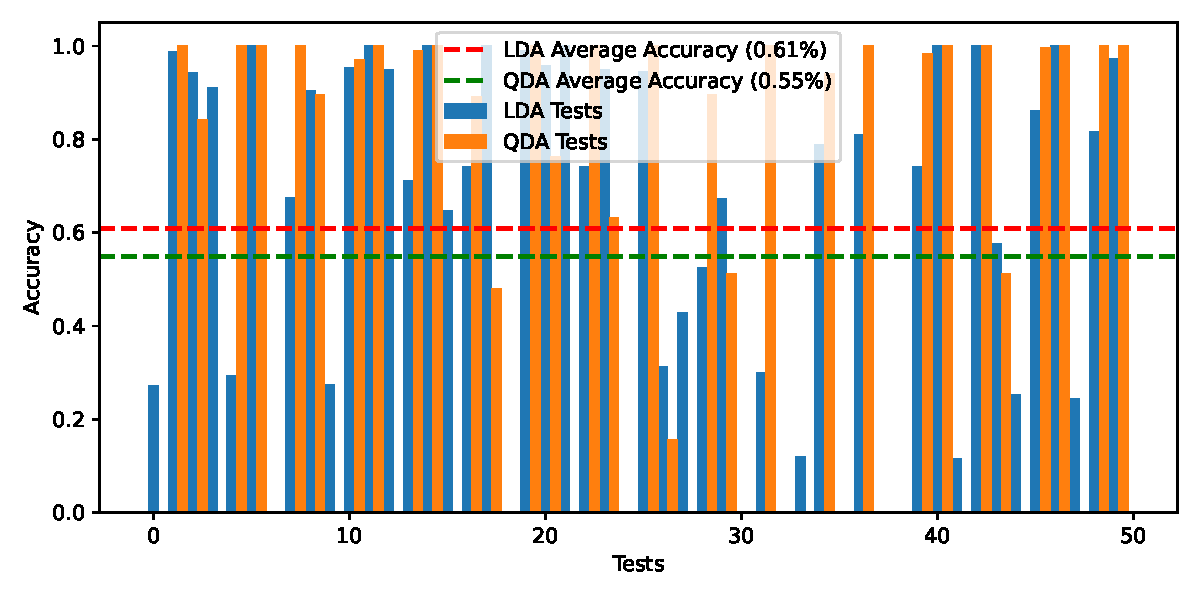
\includegraphics[width=0.99\textwidth]{lda_test.pdf}
\caption{hi}
\label{fig:lda_test}
\end{center}
\end{figure}



\begin{figure}[h]
\begin{center}
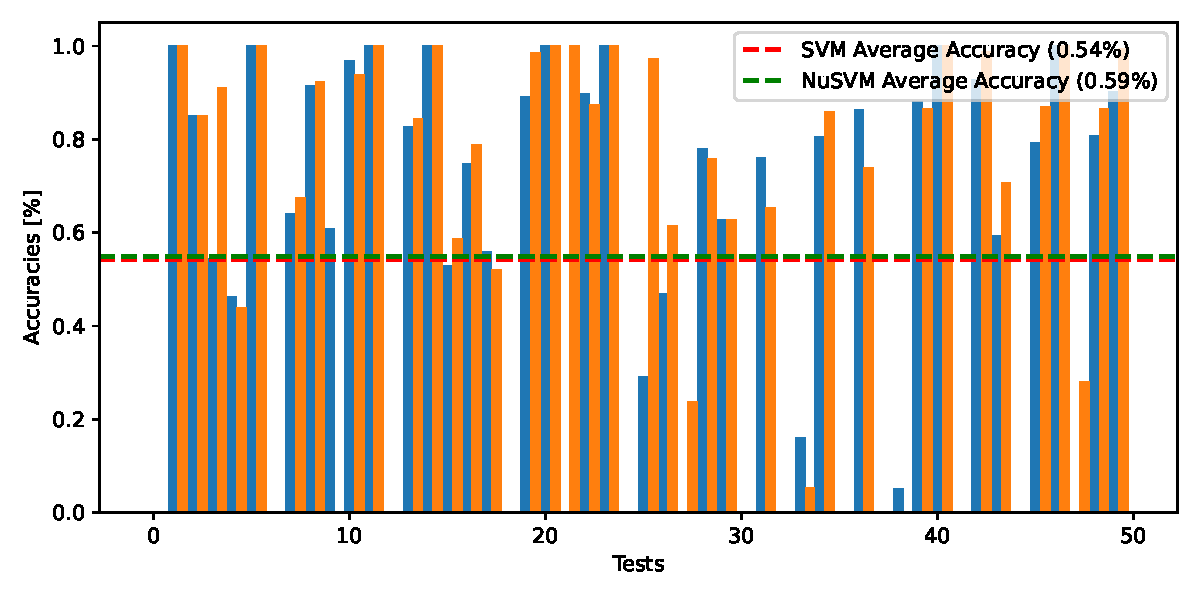
\includegraphics[width=0.99\textwidth]{svm_test.pdf}
\caption{hi}
\label{fig:svm_test}
\end{center}
\end{figure}


\subsubsection{Evaluation}


\subsection{Windowed Convolusional Neural Networks}

\subsubsection{Implementation}

%TODO: WHY CHOOSE A CNN? SELL IT LIKE A CAR!
The sEMG data used as input for regression networks is complex. The sequences of muscle activity needs to be understood by the proposed method and produced into a an output.
A network type that is ideal to understand complex meaning in, 3-dimensionary inputs is a CNN network.
%A CNN is an alternative to a MLP network that is similar in functionality is a Convoluted Neural Network (CNN).
A CNN consists of a set of Convolutional Layers that deforms inputs to abstract convolution features.
The structure is considered sparcely connected due to the convolution layers are only recieving a subset of the previous convolution features.
The feature conversion is ideal when a network needs to become robust and needs to recognize larger concepts in the input.
This functionality is especially used when the input data takes the shape of a matrix.
Once the input is convoluted to a chosen feature abstraction, it is given to a MLP strucure trained to convert the convolution features into a useable output.
%TODO: needs sources for this stuff?
%TODO: Go back and see what papers uses CNN's
CNN networks have no buildin time-based functionality, they recieve a set of inputs and produce an output.
It is possible however to represent time if the input is given in segments consisting of multiple timeframes.
Because of this, the sEMG muscle activity from the dataset is segmented into windows of a desired size, the output angles that the network should do regression towards are then chosen to be the first angle after the window.
%TODO: Images of these for better clarity!!!!
A CNN network can be used in the field of sEMG processing due to the convolution layer's ability to learn abstract formations of the sEMG data.
The network would be able to identify patterns in sEMG data and correlate them to an appropoate output.
%TODO: formations? another word?
The CNN network structure seen in figure \ref{fig:cnn_structure}.

\begin{figure}[h]
\begin{center}
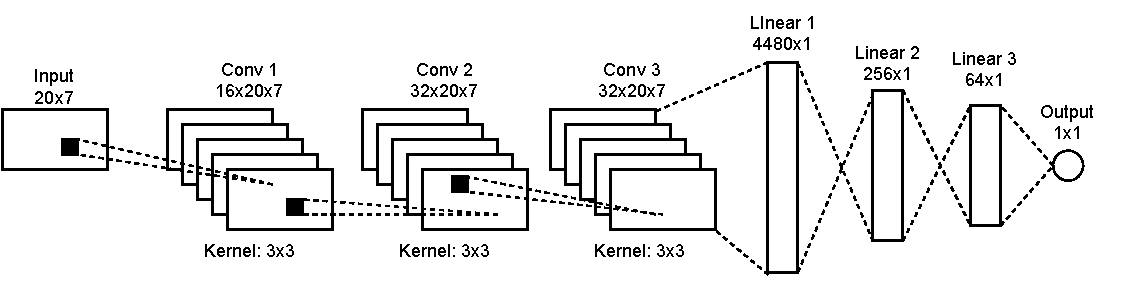
\includegraphics[width=0.99\textwidth]{cnnstructure.drawio.pdf}
\caption{The chosen CNN network structure, consisting of 3 Convolution Layers and 3 Linear layers. Network input is a window of sEMG recordings, with the purpose of regression of a finger joint angle.}
\label{fig:cnn_structure}
\end{center}
\end{figure}
%TODO: The 20 in this case refers to N samples! if i want something else than 20, change the image!

As visualized in the figure, the CNN network consists of 3 Convolution layers followed by 3 MLP layers.
The chosen CNN network structure is chosen to be simple due to the small input window of 7 muscle sensors and a window size of 20 samples.
For this reason, no pooling was used between the convolution layers.
The Convolution layers extract features up to a size of 32 using a convolution kernel with a size of [$3, 3$].
The convolution features are then flattened, to a size of $4480$, before being subject to the MLP layers that convert the extracted features into a regression prediction. 
%A CNN is trained on the network, using a window size of 40 samples were used.
%TODO: Give example of a state-of-the-art paper CNN as an alternative to mine!!!

The CNN network is trained to do regression of joint angles of the hand, because of this, the loss function is determined to be Mean Square Error (MSE) loss.
The network is trained using an Adam optimizer with a learning rate of $1\text{e}^{-4}$.
A subset of the dataset is split into a test and a validation set, and windows are extracted correlating input and output.
The output is normalized, and the input/output sets are shuffeled before training takes place.

\subsubsection{Tests \& Results}

In order to test the CNN network and assess its performance, the training MSE loss can be seen in figure \ref{fig:cnntrainvalid}.
%TODO: Make sure this graph is explained properly and is the actual image

\begin{figure}[h]
\begin{center}
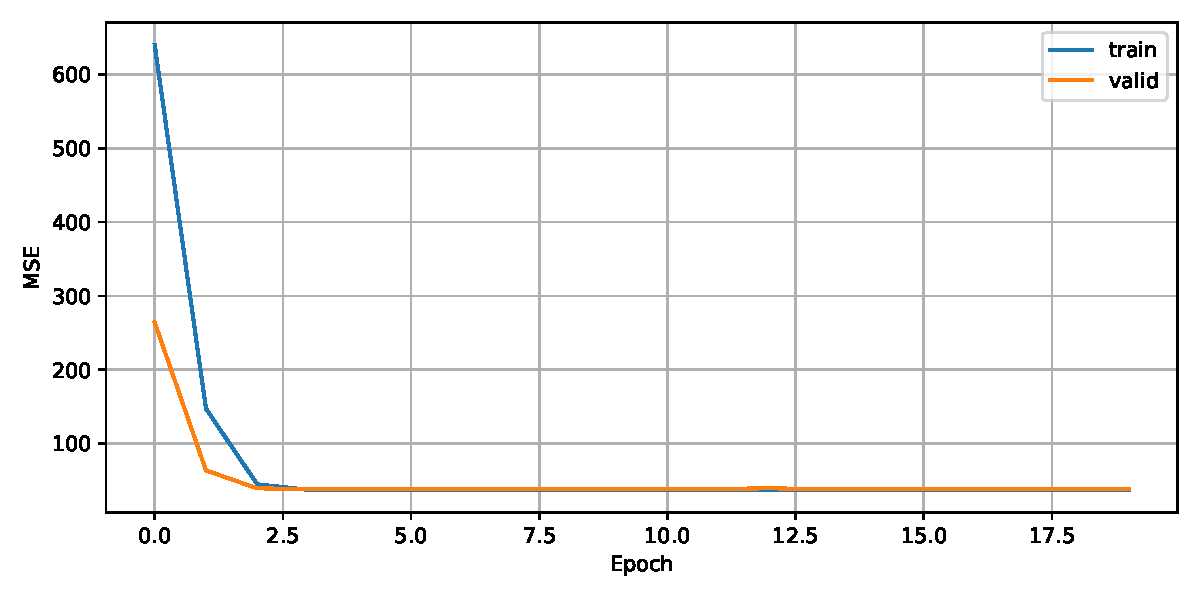
\includegraphics[width=0.8\textwidth]{cnn_trainvalid.pdf}
\caption{The Train and Validation MSE loss during training of the CNN network method.}
\label{fig:cnntrainvalid}
\end{center}
\end{figure}

The CNN network is trained with a batch size of 8 over 20 epocs, but as can be seen in the figure, the MSE loss settels at $\sim 34$ after just 3 epocs.

A random set of 50 angles that have not been trained on are taken from the dataset for testing.
The errors of the dataset are plotted, as can be seen in figure \ref{fig:cnntest}.

\begin{figure}[h]
\begin{center}
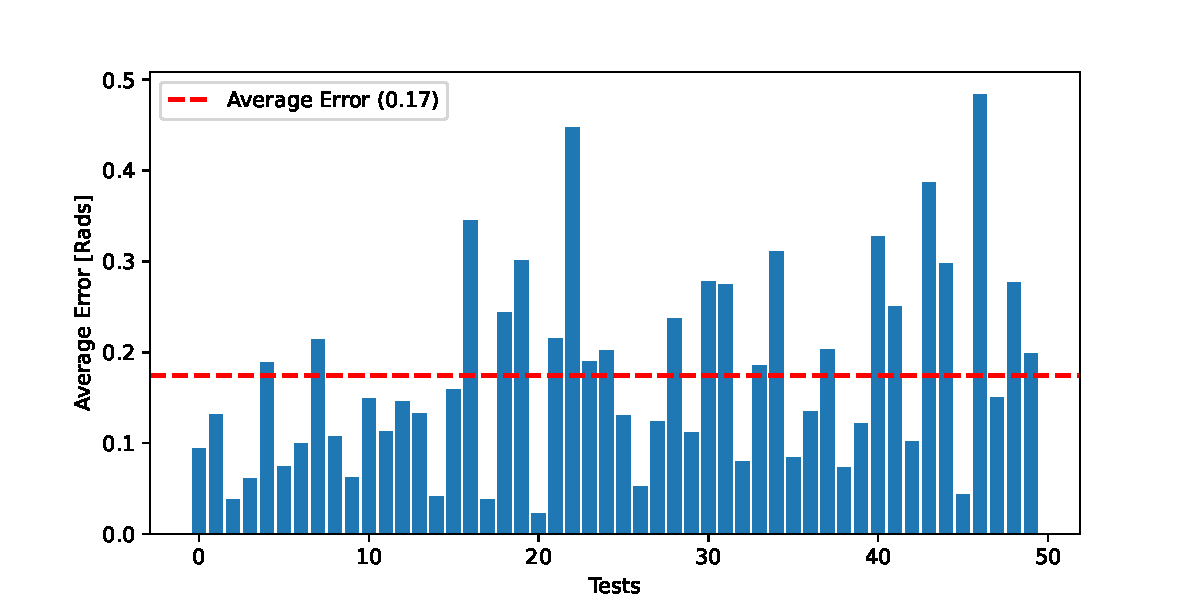
\includegraphics[width=0.99\textwidth]{cnn50test.pdf}
\caption{The errors of 50 regressions using the CNN network.}
\label{fig:cnntest}
\end{center}
\end{figure}
%TODO: What i need to do:
% Pull out 50 sets of data, do regression using my cnn model, plot their average errors in a barplot!
% This method will be my main regression test!


\subsubsection{Evaluation}

As can be seen in figure \ref{fig:cnntrainvalid}, the CNN network is able to be trained on the dataset with a validation set MSE loss of $0.34$.
The errors of the 50 test regressions in figure \ref{fig:cnntest} show that a fairly large error exists in the regressions, with an average regression error of $0.17$ Radians.
%TODO: Get the max error!

%TODO: Maybe do a average error boxplot too?


\subsubsection{Recurrent Neural Networks}

Due to sEMG data being time-based, Recurrent network types are ideal for regression predictions.
RNN networks are similar to MLP's with the main difference being that a RNN has hidden feedback  memory state that is derived from earlier inputs.
This functionality makes RNN networks ideal for concurrent, time-based systems where a sequencial input distribution needs to be converted to a output regression.  
%TODO: Alternative to concurrent -> i want something that explains a set of data in a graph!
Another use case of RNN-based regression systems are systems where responce time is critical.
The RNN network does not use a window of data, it converts the input of the current time frame, and the feedback of the previous time frame into a prediction.
Because of the hidden memory, a RNN network has a quicker response time than a window-based network.
The RNN network structure designed to predict regression of finger movements from sEMG data can be seen in figure \ref{fig:rnn_structure}.
%TODO: This one sounds nice, can it be integrated?
%The recurrent feedback loop correlates previous predictions with future predictions, allowing the network to approximate regressions per time frame.

\begin{figure}[h]
\begin{center}
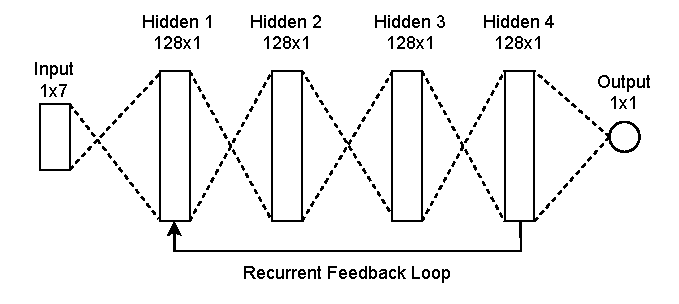
\includegraphics[width=0.8\textwidth]{rnnstructure.pdf}
\caption{The chosen RNN network structure, consisting of a input layer, 4 hidden layers with a recurrent feedback loop, and a output layer.}
\label{fig:rnn_structure}
\end{center}
\end{figure}

\subsubsection{Tests \& Results}

The RNN network is trained on the dataset \cite{kinmusdataset}, in a similar way as the RNN network, with the purpose of approximating finger angle regressions per time frame.
The RNN network is trained with a batch size of 8, with the  MSE loss function and the Adam optimizer with a learning rate of $1\text{e}^{-2}$.

In order to test the network, a random set of 50 regressions that have not been trained on are taken from the dataset.
The average errors of each regression are plotted, as can be seen in figure \ref{fig:cnntest}.

\begin{figure}[h]
\begin{center}
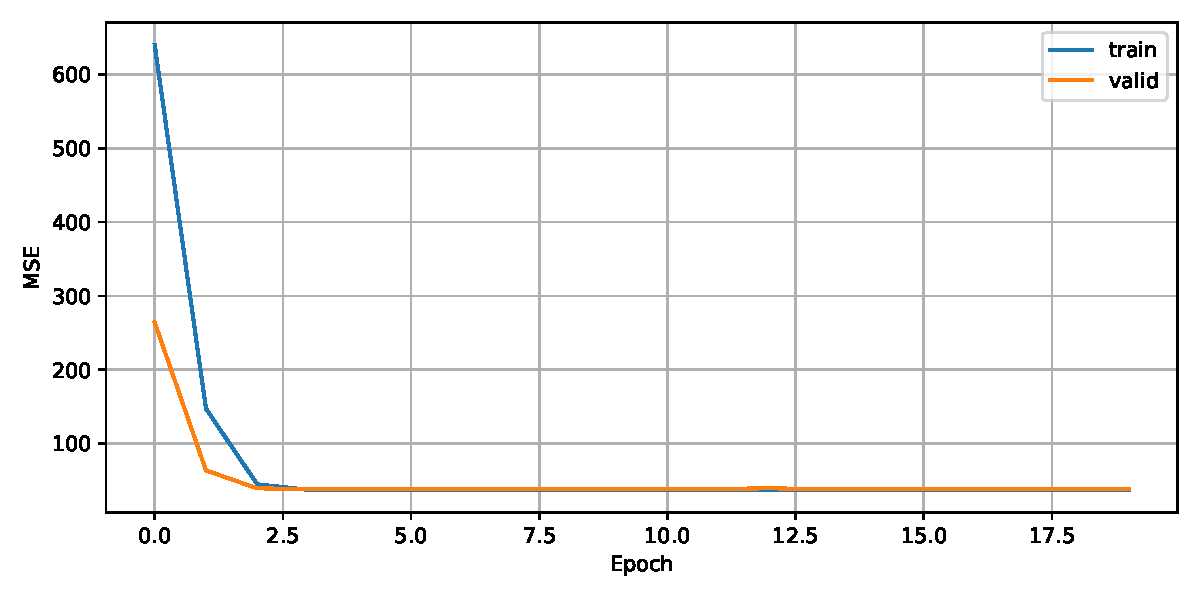
\includegraphics[width=0.8\textwidth]{cnn_trainvalid.pdf}
\caption{The errors of 50 regressions using the RNN network.}
\label{fig:rnntest}
\end{center}
\end{figure}
%TODO: What i need to do:
% Pull out 50 sets of data, do regression using my cnn model, plot their average errors in a barplot!
% This method will be my main regression test!


\subsubsection{Evaluation}

\begin{figure}[h]
\begin{center}
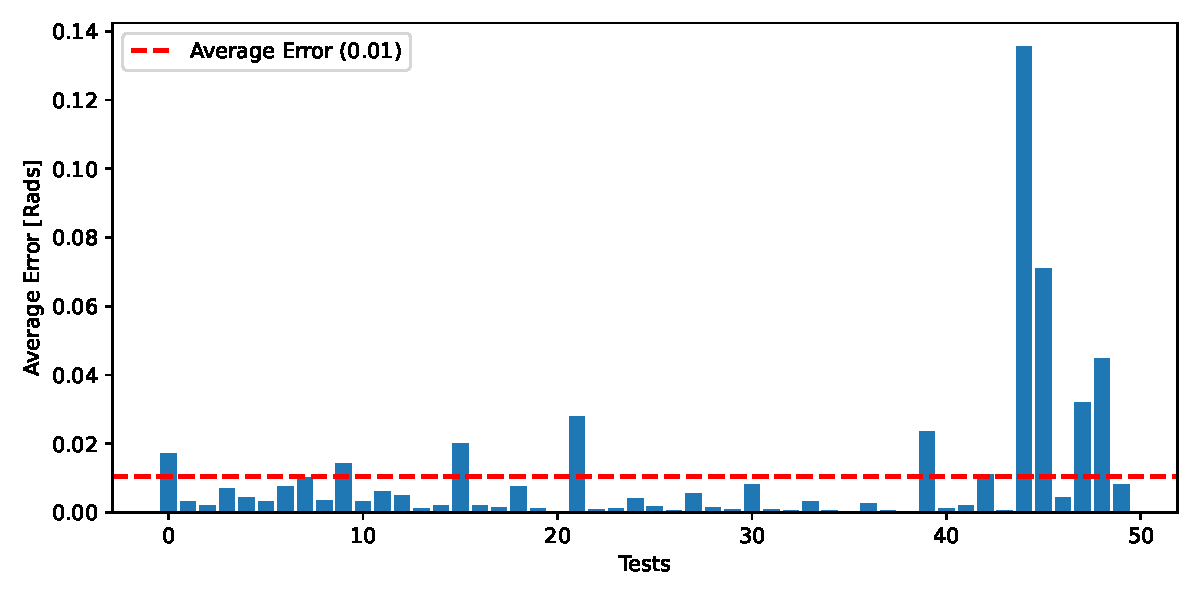
\includegraphics[width=0.99\textwidth]{rnn50test.pdf}
\caption{The errors of 50 regressions using the CNN network.}
\label{fig:rnntest}
\end{center}
\end{figure}


%As can be seen in figure \ref{fig:cnntrainvalid}, the CNN network is able to be trained on the dataset with a fairly low MSE loss.  
The errors of the 50 test regressions in figure \ref{fig:cnntest} show that a fairly small error exists in the regressions, with a maximum regression error of ?? Radians.

%TODO: Get the max error!

%TODO: Maybe do a average error boxplot too?


%TODO: Some introduction and explanation of RNN and LSTM types of networks.
%TODO: Go back and see what papers uses these.

%\subsection{(Machine Learning Algorithms)}
%%TODO: Determine what algorithms i want here
%
%\subsubsection{Types of Features for extraction}
%\textbf{Method}\\
%\textbf{Test}\\
%\textbf{Results}\\


%\subsubsection{Long-Short-Term-Memory Recurrent Neural Networks}
%TODO: Create this if you have the time..
%A variant of a RNN can contain a special kind of hidden memory called Long Short Term Memory (LSTM).
%a LSTM uses gates as a way of containing a memory.

\subsection{Comparison of Regression-based Networks}

\begin{figure}[h]
\begin{center}
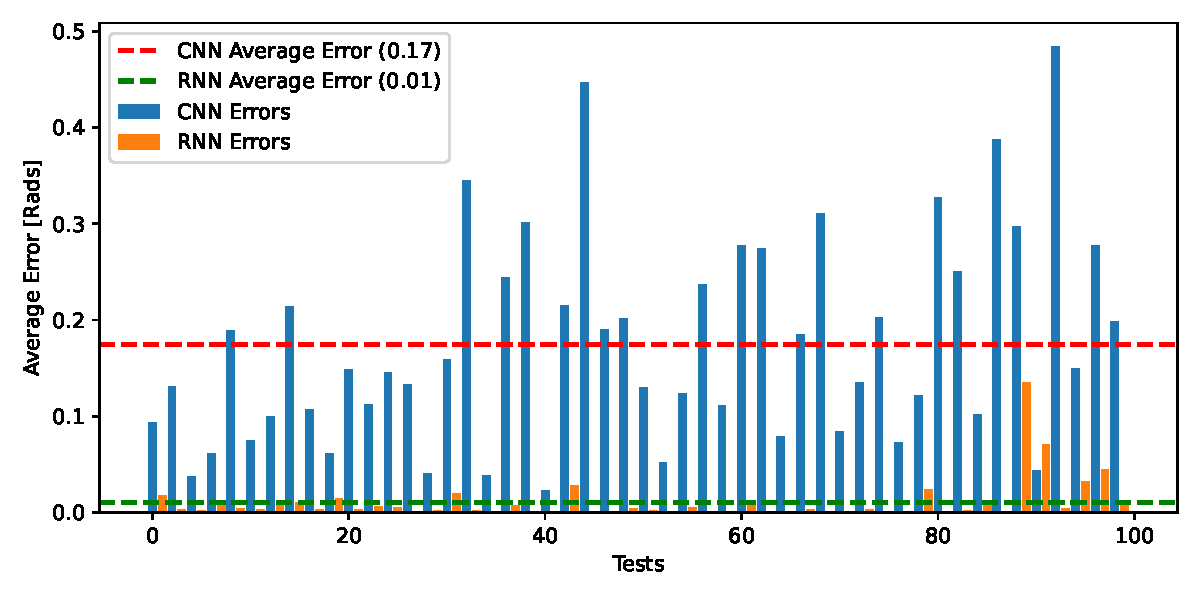
\includegraphics[width=0.99\textwidth]{regression_comparison.pdf}
\caption{hi}
\label{fig:regression_comp}
\end{center}
\end{figure}




\subsection{Feature-Based Multi Layer Perceptron Network}

Neural Networks are widely used in the field of AI.
One type of widely used neural network is a fully-connected Multi-Layer Perceptron (MLP) Network.
The MLP network is popular due to its structure and training capabilities.
A MLP consists of layers of weighted activation functions where each activation function in a layer recieves the entire previous layer's output summed up as input.
Due to the structure of a MLP, the network is capable of recieving a set of inputs and be trained to approximate a n'th degree polynomial function that relates the given inputs and outputs.
The network is trained by updating the individual weights through backpropagation with the predicted output and a ground-truth output.
The MLP network could be used to predict the relation between muscle activity and finger movements.

%In order to initially test the the dataset, a simple MLP network will be trained as a baseline for performance, and for testing the general applicability of window-based networks.


\subsection{Creation of a Dataset}

%TODO: Explain the software i made to clearn motive!
%TODO: Explain and showcase some pre-processing filters mentioned by other papers!
%TODO: Maybe here, maybe in methodology: Show how the gt angles are calculated too..

\subsection{Useability of the Simulated Prosthetic Hand}

Existing prosthetic hand simulations are not possible to get access to, as explained in section \ref{sec:hand_alternatives}, they are either unavailable through deprecation or pay-to-acces by buying a real prosthetic.
Due to non-availability of prosthetic hand simulations, it was chosen that through this thesis, a open source prosthetic hand needed to be created for testing of the algorithms developed as part of this project.
The prosthetic hand created for this thesis can be seen in section \ref{sec:prost_sim}.
The prosthetic was designed to be as anatomically similar as a real hand as possible.
This was done in order to accurately simulate the movement of a real hand.
%TODO: Is this intro good?

\subsubsection{Anatomical Assessment and Maneuverability}

The useability and moveability of the simulated prosthetic hand needs to be assessed.

\textbf{Method}\\
As an initial test, it is reasonable to test if the hand is able to acheive the end poses of the grip types from section \ref{sec:dataset} table \ref{tab:grips}. 

\textbf{Test \& Results}\\

The hand was manually posed into all 4 grip types, and visually compared, as can be seen in figure  \ref{fig:hand_pose_test}.

%TODO: Needs to be a figure of figures!
\begin{figure}[h]
\begin{center}
\includegraphics[width=0.8\textwidth]{example-image-a}
\caption{Example figure text}
\label{fig:hand_pose_test}
\end{center}
\end{figure}


Based on a visual comparison of figure \ref{fig:hand_pose_test}, it can be concluded that the prosthetic hand is able to be posed similarly to the real-life refrence.
It can be seen how the prosthetic is porpotionally correct and thus also allows for accurate posing when posed manually.

\subsubsection{Posing based on Network Output}

As a result of testing different network types and their applicability for creating suitable motorcontrol output for a prosthetic hand, it would be ideal to test the network output on the prosthetic simulation.
For full video see appendix ??.
%TODO: Insert appendix here

\textbf{Method}\\

\textbf{Test \& Results}\\



%\subsection{Method 1: Windowed CNN}
%\subsection{Test 1: Windowed CNN}
%\subsection{Results 1: Windowed CNN}
%\subsection{Method 2: RNN}
%\subsection{Test 2: RNN}
%\subsection{Results 2: RNN}


%TODO: see Zhaolong2021 (page 10) for example of how to compare MSE for different neuron amounts, even for multiple subjects!

\end{document}
